\documentclass[a4paper,article]{article}

\usepackage[utf-8]{inputenc}
\usepackage[russian]{babel}

\usepackage{amsmath,amssymb}
\usepackage{graphicx}

\begin{document}
\tableofcontents
\section{Сферические координаты}
$\lambda \in [0,2\pi]$ - долгота. $\phi \in [-\pi/2,\pi/2]$ - широта.

\begin{equation*}
\begin{split}
x = cos \lambda cos \phi, \\
y = cos \lambda sin \phi, \\
z = sin \phi. 
\end{split}
\end{equation*}

Обратное преобразование:
\begin{equation*}
\begin{split}
\phi = arcsin z, \\
\lambda = arccos \frac{x}{\sqrt{x^2+y^2}}, \text{ при } y \ge 0,\\
\lambda = 2 \pi - arccos \frac{x}{\sqrt{x^2+y^2}}, \text{ при } y < 0.
\end{split}
\end{equation*}

\subsection{Построение сетки}
\subsubsection{Полная сфера}
Возьмем икосаэдр. Каждое ребро икосаэдра разделим пополам и получившуюся точку спроектируем на сферу. С получившимся многогранником можно проделать ту же самую процедуру. На каждом шаге алгоритма шаг сетки уменьшается вдвое.

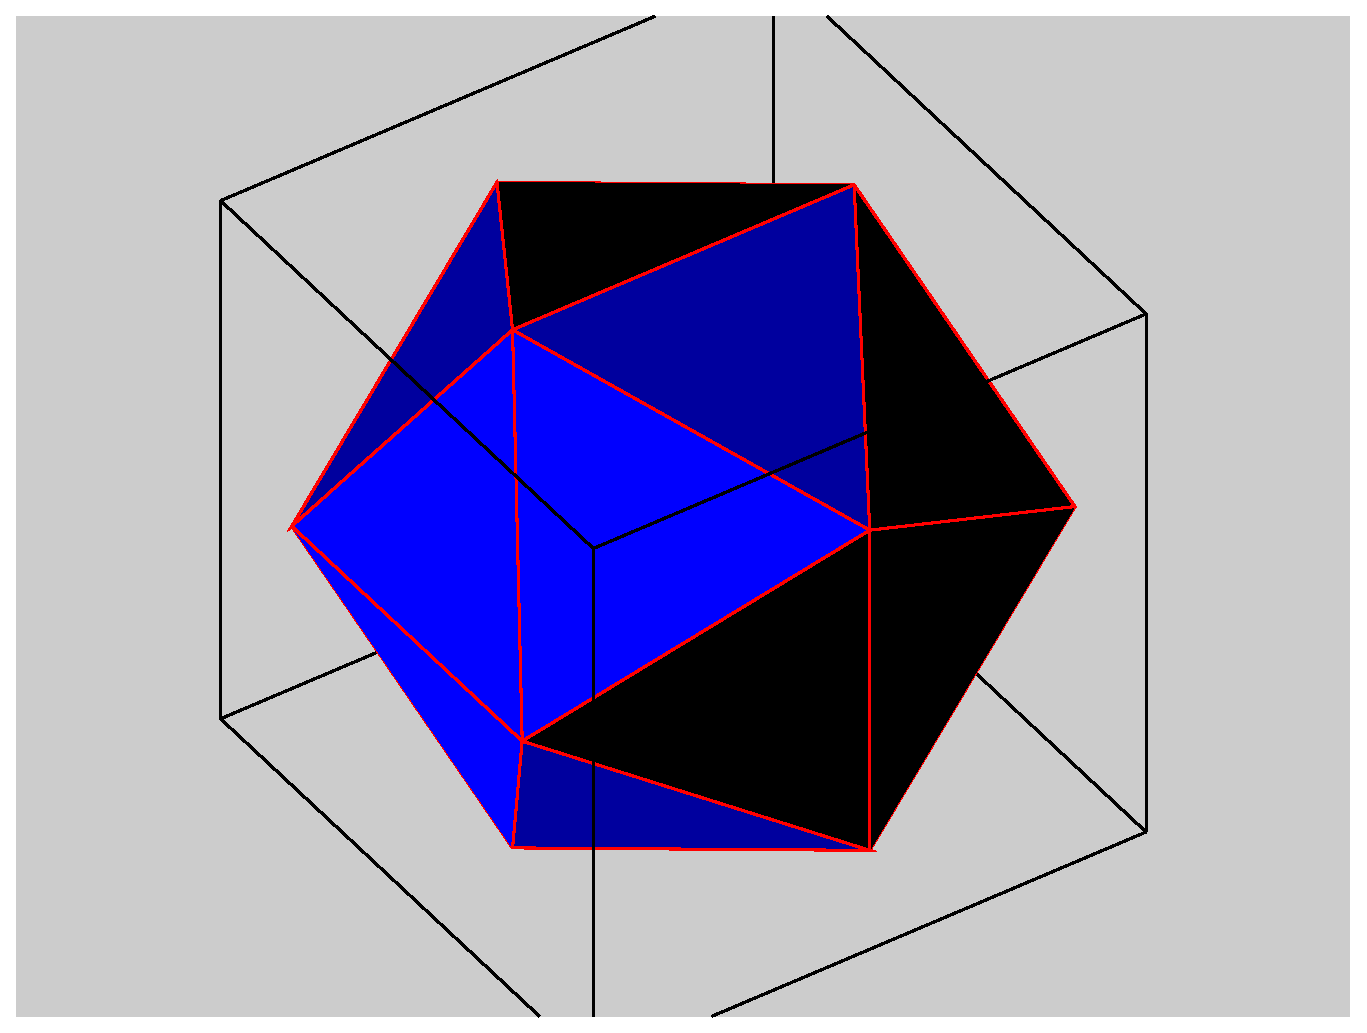
\includegraphics[scale=0.5]{icosahedron.eps}

\subsubsection{Полусфера}
Алгоритм аналогичен, только вместо икосаэдра берем трапецию:

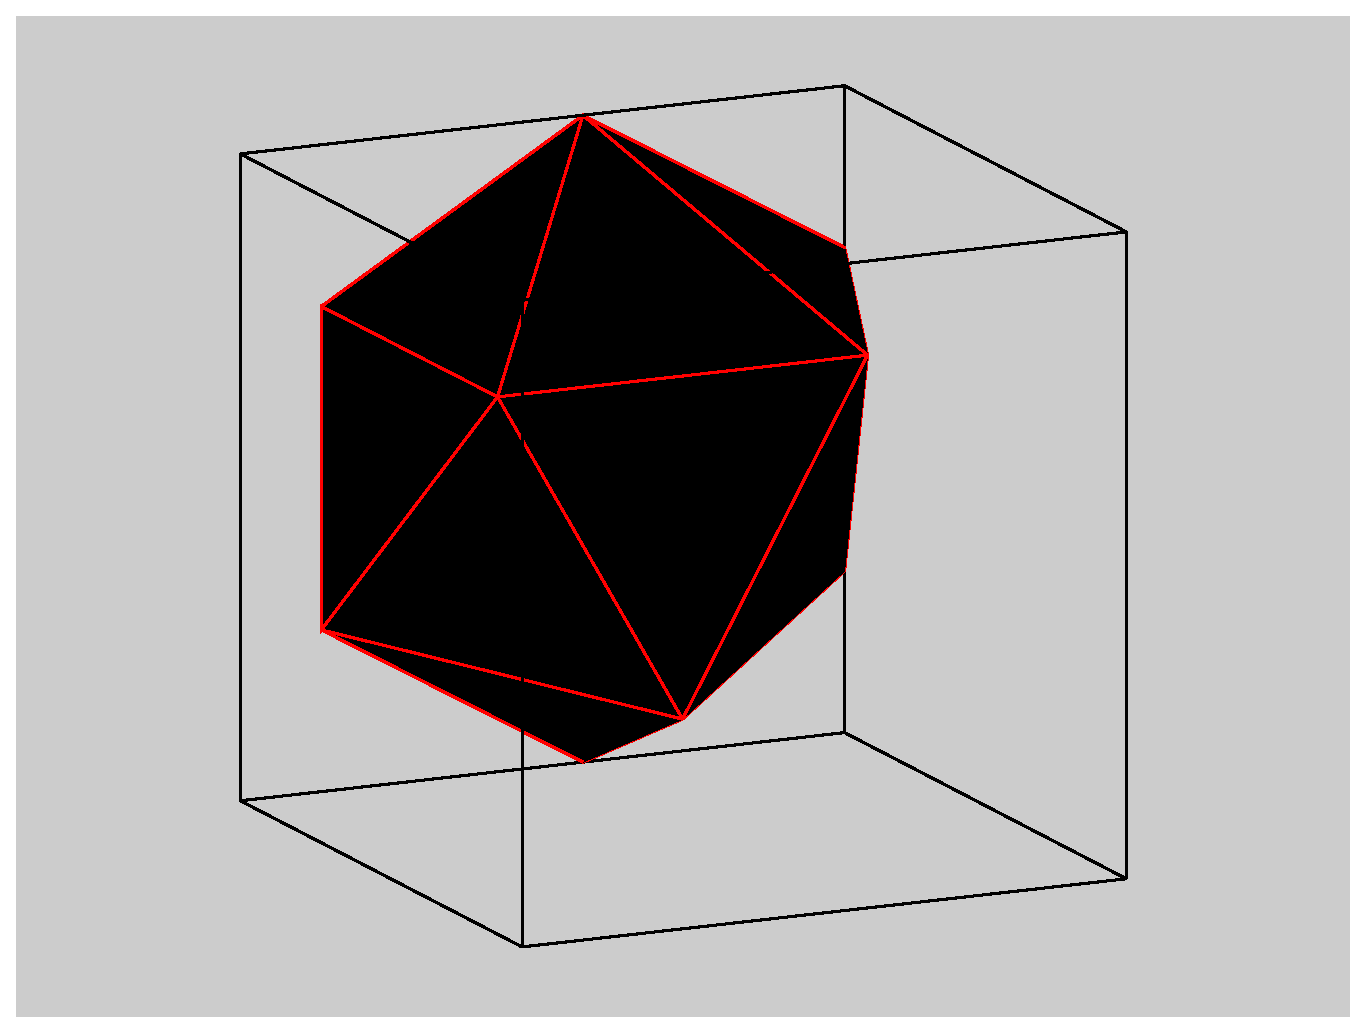
\includegraphics[scale=0.5]{hemisphere.eps}

\subsubsection{Область сферы}
Алгоритм аналогичен, достаточно выбрать первоначальное разбиение облати на треугольники.
Пример области $[\lambda,\phi]=[0,\pi]\times[0,\pi/4]$:

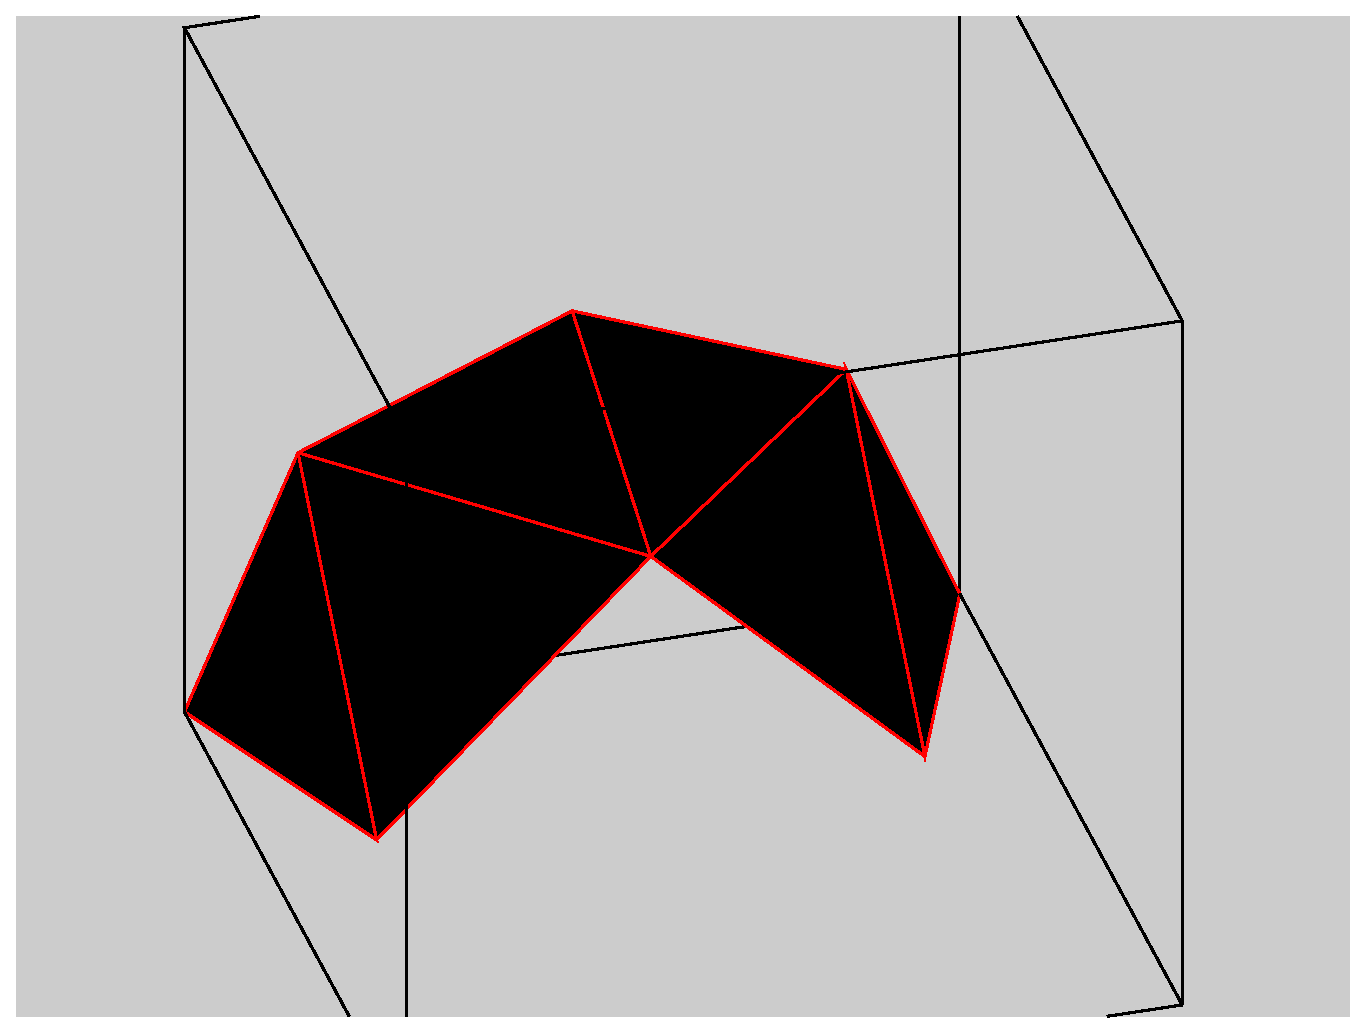
\includegraphics[scale=0.5]{test.eps}

см. файл icosahedron.cpp:
\begin{itemize}
\item Построение начального разбиения: build\_icosahedron, build\_hemisphere, build\_test
\item Проектирование на сферу: normalize
\item Измельчение сетки: iterate\_mesh
\item Вывод сетки в stdout: print\_mesh
\end{itemize}
исполняемый файл: sphere:
\begin{verbatim}
usage: ./sphere --type [full|half] --coord [local|global] --iter [number]
--type
   full -- fulsphere
   half -- hemisphere
   test
--coord
   local -- (u,v)
   global -- (x,y,z)
--iter
   number -- number of iterations
\end{verbatim}

\section{Оператор Лапласа}
\begin{equation*}
\Delta u(\phi, \lambda) = \frac{1}{cos \phi}\frac{\partial}{\partial \phi} cos \phi u(\phi, \lambda)+\frac{1}{cos^2 \phi}\frac{\partial^2}{\partial\phi^2}u(\phi, \lambda)
\end{equation*}

Дифференциальная задача:
\begin{equation*}
\Delta u(\phi, \lambda) = f(\phi, \lambda)
u\|_{\partial\Omega} = u_0
\end{equation*}

Численная задача:
\begin{equation*}
\begin{split}
(\frac{1}{cos\psi}\frac{\partial}{\partial \phi} \phi_i, cos\phi \frac{\partial}{\partial \phi} \phi_j) = -(f, \phi_j), \forall j, \forall i, \text{ для внутренних узлов } \\
u = u_0 \phi_i, \text { для граничных узлов, }
\end{split}
\end{equation*}
где $\phi_i$, $\phi_j$ - базисные функции.

Скалярное произведение:
\begin{equation*}
(u, v) = \int_\Omega u v ds = \int\int_\Omega u v cos(\phi)d\lambda d\phi.
\end{equation*}

Система уравнений:
\begin{equation*}
\sum_j x_j \sum_{k: \{j\in\bigtriangleup_k, i\in\bigtriangleup_k\}}\int_{\bigtriangleup_k}\frac{1}{cos\psi}(\frac{\partial}{\partial \phi} \phi_i) cos\phi (\frac{\partial}{\partial \phi} \phi_j) ds = \sum_{k:\{i\in\bigtriangleup_k\}}\int_{\bigtriangleup_k}f \phi_j ds,
\end{equation*}
где
\begin{equation*}
u(\phi,\lambda)=\sum_i x_i \phi_i(\phi, \lambda),\\
f(\phi,\lambda)=\sum_i f_i \phi_i(\phi, \lambda).
\end{equation*}

см. файл sphere\_laplace.cpp

\subsection{Базисные  функции}
Используются линейные базисные функции. Каждая базисная функция $\phi_i$ равна единице в узле с номером $i$ и нулю в остальных узлах. Функция отлична от нуля на треугольниках, содержащих узел с номером $i$.
Три базисные функции на треугольнике с координатами $x_1,x_2,x_3, y_1,y_2,y_3$:
\begin{equation*}
\begin{split}
\psi_1=(x-x_2)(y_3-y_2)-(y-y_2)(x_3-x2),\\
\psi_2=(x-x_1)(y_3-y_1)-(y-y_1)(x_3-x1),\\
\psi_3=(x-x_1)(y_2-y_1)-(y-y_1)(x_2-x1).
\end{split}
\end{equation*} 
\begin{equation*}
\phi_i=\frac{\psi_i}{\psi_i(x_i,y_i)}
\end{equation*}

см. файл mke.cpp: функции elem1, elem1\_inner.
Каждая функция представляется полиномом от двух переменных $(x,y)$.

см. файл polynom.h: класс Polynom содержит вектор коэффициэнтов, доступны все операции с полиномами. Поддерживаются только полином от $(x)$ и от $(x,y)$.

\subsubsection{Интегрирование  полиномов} 
mke.cpp: функция integrate - вычисление интегралов вида:
\begin{equation*}
\begin{split}
\int_\bigtriangleup P(x,y) dx dy,\\
\int_\bigtriangleup P(x,y) cos(x) dx dy,\\
\int_\bigtriangleup P(x,y) / cos(x) dx dy.
\end{split}
\end{equation*}

util.cpp: функция trapezoid\_integrate - вычисление интегралов вида:
\begin{equation*}
\begin{split}
\int_\bigtriangleup x^k y^n dx dy\text { - считается аналитически }, \\
\int_\bigtriangleup x^k y^n cos x dx dy\text{ - используется квадратура Гаусса-Кронрода 15 } ,\\
\int_\bigtriangleup \frac{x^k y^n}{cos x} dx dy\text{ - используется квадратура Гаусса-Кронрода 15 }.
\end{split}
\end{equation*}

\section{Сборка и запуск}
\begin{verbatim}
cmake -DCMAKE_BUILD_TYPE=Release
make
./sphere --type test --iters 5 --coord local > mesh.txt
./test_slaplace mesh.txt
\end{verbatim}

\begin{thebibliography}{999}
\bibitem{bogach3} Богачев К. Ю., {\it  Практикум на ЭВМ.  Методы
    приближения функций, 3-е изд.}// M.:Изд-во
  механико-математического факультета МГУ. 2002.

\end{thebibliography}

\end{document}

